% Author: Izaak Neutelings (July, 2017)
% based on code from a friend
\documentclass[border=1pt,tikz]{standalone}

\usepackage{amsmath} % for \dfrac
\usepackage{tikz}
\usepackage{calc} % for simple arithmetic
\tikzset{>=latex} % for LaTeX arrow head



\begin{document}



% LOGARITHMIC SCALE
\large
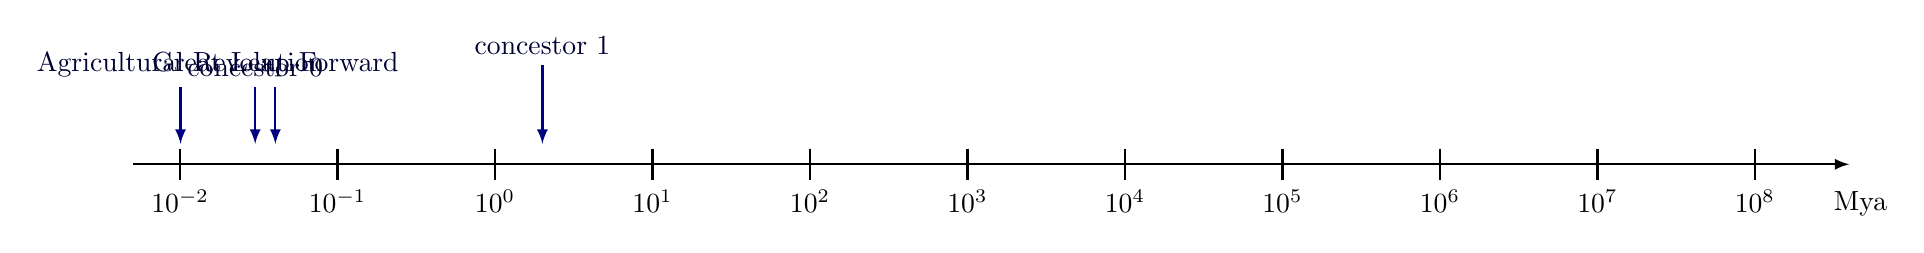
\begin{tikzpicture}[]
  
  % limits
  \def\nOne{-2}
  \def\w{20}      % width of axes 
  \def\n{10}      % number of decades
  \def\noffset{1} % offset labels
  \def\nskip{1}   % skip number
  \def\la{2.00}   % arrow length
  \def\lt{0.20}   % tick length
  \def\ls{0.15}   % tick length (skipped)
  
  % help functions
  \def\mylog(#1){{(log10(#1)-\nOne)*\w/\n}}
  \def\arrowLabel(#1,#2,#3,#4){
    \def\xy{(#1)}; \pgfmathparse{int(#2*100)};
    \ifnum \pgfmathresult<0
      \def\yyp{{(\lt*(-0.10+#2))}}; \def\yyw{{(\yyp-\la*\lt*#3)}}
      \draw[<-,thick,black!50!blue,align=center]
        (\mylog(\xy),\yyp) -- (\mylog(\xy),\yyw)
        node[below,black!80!blue] {#4};
    \else
      \def\yyp{{(\lt*(0.10+#2)}}; \def\yyw{{(\yyp+\la*\lt*#3)}}
      \draw[<-,thick,black!50!blue,align=center]
        (\mylog(\xy),\yyp) -- (\mylog(\xy),\yyw)
        node[above,black!80!blue] {#4};
    \fi
  }
  \def\arrowLabelRed(#1,#2,#3,#4){
    \def\xy{{(#1-\nOne)*\w/\n}};
    \def\yyp{{(\lt*(-0.10+#2))}}; \def\yyw{{(\yyp-\la*\lt*#3)}}
    \fill[red,radius=2pt] (\xy,0) circle;
    \draw[<-,thick,black!25!red,align=center]
      (\mylog(\xy),\yyp) -- (\mylog(\xy),\yyw)
      node[below,black!40!red] {\strut#4};
  }
  
  % axis
  \draw[->,thick] (-\w*0.03,0) -- (\w*1.06,0)
                  node[right=4pt,below=6pt] {Mya};
  
  % ticks
  \foreach \tick [evaluate={\x=\tick*\w/\n;
                            \c=(mod(\tick-\noffset,\nskip)==0);}]
                 in {0,1,...,\n}{
    \def\dec{\the\numexpr \nOne+\tick \relax}
	\if\c1
	  \draw[thick] (\x,\lt) -- (\x,-\lt) % ten tick
	               node[below] {$10^{\dec}$}; % label
	\else
      \draw[thick] (\x,\ls) -- (\x,-\ls); % ten tick
	\fi
  }
  
  % label
  \arrowLabel(0.01,1.2,1.8,Agricultural Revolution) % 10,000 y = 0.01 Mya
  \arrowLabel(0.04,1.2,1.8,Great Leap Forward)      % 40,000 y = 0.04 Mya
  \arrowLabel(0.03,1.2,1.8,concestor 0)             % 50,000 y = 0.05 Mya
  \arrowLabel(   2,1.2,2.5,concestor 1) % 
  
\end{tikzpicture}

  

\end{document}
